\documentclass[aspectratio=169,t]{beamer}
\usepackage[utf8]{inputenc}
\usepackage[T1]{fontenc}
\usepackage[export]{adjustbox}
\usepackage{amssymb}


\title{Programmierung 1}
\date{SS 2020}
\author[PWD]{Prof. Dr.-Ing. Piotr Wojciech Dabrowski}
\titlegraphic{Bilder/logo.png}

\usepackage{HTWBeamerTemplate/beamerthemeHTW}
%\setbeameroption{show notes on second screen}

\subtitle{1: Allgemeines}
\addbibresource{sources_01.bib}
\begin{document}

\setbeamertemplate{footline}[first]

\begin{frame}[noframenumbering]
    \titlepage
    \begin{textblock}{10}(4.75,15)
        \cite{logo}
    \end{textblock}
\end{frame}

\setbeamertemplate{footline}[presentationbody] 

\begin{frame}{Vorstellung}
	\begin{itemize}
		\item Kontakt:
		\begin{itemize}
			\item Piotr.Dabrowski@htw-berlin.de
			\item Sprechstunde: Montag 10-11, WH C 614
		\end{itemize}
		\item Background
		\begin{itemize}
			\item Medizinische Biotechnologie + Informatik, dann Bioinformatik
			\item Analyse von Next Generation Sequencing-Daten
			\item Aufbau der Bioinformatik Core-Facility am Robert Koch-Institut
			\item Exkurse in BMF, BMI $\rightarrow$ Projekte bei Interesse möglich
			\item Potentielles Wiedersehen: Gesundheitsinformatik
			\item Seit WS 2019/2020 an der HTW, seit SS 2020 Programmierung 1
		\end{itemize}
	\end{itemize}
\end{frame}

\begin{frame}{Modalitäten}
	\begin{itemize}
		\item 2 SWS Vorlesung
		\begin{itemize}
			\item Kein Skript, viel Tafel $\rightarrow$ Mitschreiben empfehlenswert
			\item ...Aber: Sowieso nicht klausurrelevant.
			\item Fragen bitte immer sofort!
		\end{itemize}
		\item 2 SWS Übung
		\begin{itemize}
			\item Gruppe A: Frau Ursula Rehbein, Zug 1: Ich
			\item Betreutes Programmieren: Umsetzen des Vorlesungsstoffes
			\item Hausaufgaben (Voraussetzung für Prüfungszulassung!)
			\item Musterlösungen für ausgewählte Hausaufgaben
		\end{itemize}
	\end{itemize}
	Gesamtaufwand: 6 Credits = 180 Stunden\\
	Bei 16 Wochen je 3 Stunden UE + VL sind das 8 Stunden Selbststudium/Woche!
\end{frame}

\begin{frame}{Hausaufgaben}
	\begin{itemize}
		\item Meistens alle 2 Wochen
		\item Zu Hause zu lösen
		\item Elektronisch über https://moodle.htw-berlin.de abzugeben
		\begin{itemize}
			\item Jeden Abgabetermin beachten! Abgabe mehr als 15 Minuten später = 0 Punkte!
			\item Identische Lösungen (auch teilweise) = 0 Punkte!
			\item Gruppenarbeit: Informationen in der Übung
		\end{itemize}
		\item Für Klausurzulassung: Mindestens 75\% der Hausaufgaben-Punkte (Prüfungsvorleistung)
		\item Punkte für Hausaufgaben nicht zwischen Semestern übertragbar
	\end{itemize}
\end{frame}

\begin{frame}{Prüfung}
	Notwendig für die Teilnahme:
	\begin{itemize}
		\item Mindestens 75\% der Hausaufgaben-Punkte
		\item 6. Kyu auf https://www.codewars.com (Modalitäten: nächste Woche)
		\item Anmeldung im LSF (https://lsf.htw-berlin.de) im vorgegebenen Zeitraum
		\item Personalausweis oder Reisepass zur Vorlage bei der Prüfung
	\end{itemize}
	Es wird eine elektronische Klausur am Rechner geschrieben: Nur Programmieraufgaben (100\% der Note)!\\
	Vorsicht: Andere machen das anders!
\end{frame}

\begin{frame}{Laborordnung}
	Laborordnung im Internet: https://www.youtube.com/watch?v=edR-4BHWWZo\\
	Ausgewählte Punkte:
	\begin{itemize}
		\item Keine private/kommerzielle Nutzung (massiv ausgebucht!)
		\item Kein Umsöpseln, keine eigenständige Software-Installation
		\item Kein Essen, Trinken, Rauchen
		\item Dateien zusätzlich sichern, keine Garantie für Dateien auf Labor-PCs/Dateiserver
		\item Arbeit außerhalb der regulären Öffnungszeiten: Schlüssel im Servicepoint im Gebäude B
	\end{itemize}
\end{frame}

\begin{frame}{Ablauf - allgemein und heute}
	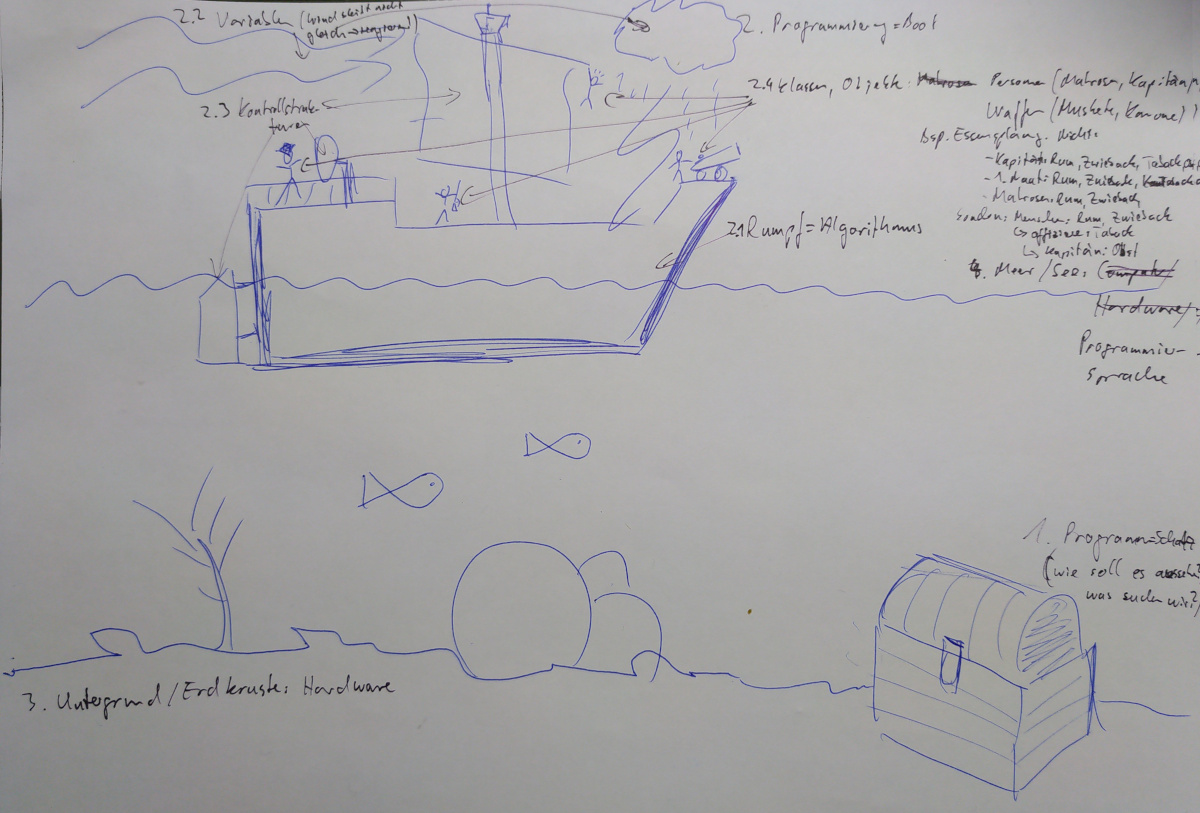
\includegraphics[height=0.7\textheight]{Bilder/VL-Bild.jpg} Heute: Ab- und auftauchen
\end{frame}

\begin{frame}{Programmierung}
	Programmierung: Computern erklären, was sie tun sollen. \\Zu beachten: Computer
	\begin{itemize}
		\item sind sehr schnell
		\item nehmen alles wörtlich
		\item denken nicht mit
	\end{itemize}
	Aufgabe der Programmierer: Komplexe Problemlösungen so in kleine Schritte aufbrechen, dass ein Computer sie durchführen kann = \textbf{Algorithmen} schreiben.\\
	Dazu notwendig:
	\begin{itemize}
		\item Die richtige Art, zu denken
		\item Viel Übung - Können ist hier wichtiger als Wissen! $\rightarrow$ Vorlesungsaufbau (...braucht man die Vorlesung überhaupt?)
	\end{itemize}
\end{frame}

\begin{frame}{Beispiel}
	Sagen Sie mir, wie ich die Tür öffnen kann!\\Ich verstehe:
	\begin{itemize}
		\item Drehen nach <links, rechts> um <wieviel> Grad
		\item Gehen nach <vorne, hinten> um <wieviel> Schritt
		\item Arm auf der <rechten, linken> Seite um <wieviel> Grad <heben, senken>
		\item Greifen mit der <rechten, linken> Hand
		\item Loslassen mit der <rechten, linken> Hand
	\end{itemize}
	Jeder, der den Ball hat, sagt eine Anweisung\\Freiwillige Hilfe: Algorithmus aufschreiben.
\end{frame}

\begin{frame}{Von Lösungsiungsidee zu Programm}
	Lästige Schreibweise im Beispiel $\rightarrow$ Konventionen, wie Anweisungen geschrieben werden = \textbf{Syntax}. Beispiel:
	\begin{itemize}
		\item ``nach'', ``um'', ``Grad'' etc. weglassen: ``Drehen nach links um 10 Grad'' $\rightarrow$ ``Drehen links 10''
		\item Zur Lesbarkeit ein paar Trennzeichen einführen: ``Drehen links 10'' $\rightarrow$ ``Drehen(links, 10)''
		\item Klar machen, wann ein Befehl beendet ist und der nächste anfängt: ``Drehen(links, 10)'' $\rightarrow$ ``Drehen(links, 10);''
	\end{itemize}
	$\rightarrow$ Übersetzung des Algorithmus in Programmcode
	\\Vokabular zum einfacheren Unterhalten: \textbf{Funktionen} und \textbf{Argumente}
\end{frame}

\begin{frame}{Für wen machen wir das?}
	Computer haben aber keine Arme oder Beine - siehe schematischer Computeraufbau (CPU, RAM mit Programm + Daten).\\
	Sie verstehen also kein ``Drehen'' etc., sondern im Grunde nur:
	\begin{itemize}
		\item Verschieben(was, wohin) \textit{(MOV src dest)}
		\item Addieren(was, zuWas) \textit{(ADD src dest)}
		\item SpringeWennRegisterNichtNull(register, sprungWeite) \textit{(JNZ reg diff)}
	\end{itemize}
	Jedes Argument kann sein: \%Register, \$Wert, (Speicheradresse)\\
	Das reicht aber (siehe Computeraufbau)! Beispiele:
	\begin{itemize}
		\item Zwei Zahlen addieren
		\item Zahl mit 3 (ohne JNZ)/einer anderen Zahl (mit JNZ) multiplizieren
		\item Bild auf Bildschirm anzeigen
	\end{itemize}
\end{frame}

\begin{frame}[t,fragile]{Zwei Zahlen addieren}
	Zahlen in Speicheradressen 1 und 2, Ergebnis soll in Speicheradresse 3 stehen
	\lstset{language=[x86masm]Assembler,texcl=true}
	\begin{lstlisting}
mov %Register1 (1)
mov %Register2 (2)
add %Register2 %Register1
mov %Register2 (3)
	\end{lstlisting}
	...Wie mache ich daraus eine Multiplikation von (1) mit \$3?
\end{frame}

\begin{frame}[t,fragile]{Zahl mit 3 multiplizieren}
	Zahl in Speicheradresse 1, Ergebnis soll in Speicheradresse 3 stehen
	\lstset{language=[x86masm]Assembler,texcl=true}
	\begin{lstlisting}
mov %Register1 (1)
mov %Register2 (1)
add %Register2 %Register1
add %Register2 %Register1
mov %Register2 (3)
	\end{lstlisting}
	...Wie mache ich daraus eine Multipliktion von (1) mit (2)?
\end{frame}

\begin{frame}[t,fragile]{Zahlen multiplizieren}
	Zahlen in Speicheradressen 1 und 2, Ergebnis soll in Speicheradresse 3 stehen
	\lstset{language=[x86masm]Assembler,texcl=true}
	\begin{lstlisting}
mov %Register1 (1)
mov %Register2 (1)
mov %Register3 (2)
add %Register2 %Register1
add %Register3 $-1
jnz %Register3 $-2
mov %Register2 (3)
	\end{lstlisting}
	...Wie gebe ich den Wert - z.B. auf 7-Segment-Anzeige - aus? (das wird mit nur 3 Befehlen eklig $\rightarrow$ je Wert1 Wert2 Sprungweite, jmp Sprungweite, Bitmaps)\\
	...Wie sieht das tatsächlich im Rechner aus? $\rightarrow$ Maschinencode
	...Wie baue ich ``Drehen(Richtung, Winkel)'' damit?
\end{frame}

\begin{frame}{Programmiersprachen}
	Aufgabe der Programmiersprache: Programmcode statt Maschinencode schreiben.
	\\Man kann mit Assembler programmieren... Aber will man es?
	\\Höhere Programmiersprachen:
	\begin{itemize}
		\item Abstrahieren Hardware-Details auf das nötige Level
		\item Bieten Funktionen für häufige Aufgaben 
	\end{itemize}
	Wie viele Programmiersprachen gibt es?\\
	\only<2->{Aktuelle Wikipedia-Liste der Programmiersprachen: ca. 1470. Warum gibt so viele?}
\end{frame}

\begin{frame}{Java}
	\begin{itemize}
		\item Sehr populäre Sprache
		\item Compiliert (Programmcode \only<2->{$\rightarrow$ Bytecode }$\rightarrow$ Maschinencode)
		\item<2-> Mit virtueller Maschine (``Compile once, run everywhere'')
	\end{itemize}
\end{frame}

\begin{frame}{Kontrollstrukturen}
%	Frage: Reichen Funktionen und Argumente, um jedes Problem zu lösen? Falls nein, was fehlt?
\end{frame}

\begin{frame}{Beispiel weiter}
	\begin{itemize}
		\item Funktioniert das nochmal (-> Startbedingungen oder Berechnungen)
		\item Für Berechnungen: Werte -> Variablen -> Datentypen etc.
	\end{itemize}
\end{frame}

\begin{frame}[allowframebreaks]{Quellenangaben}
    \printbibliography
\end{frame}

\begin{frame}{Lizenz}
    \begin{center}
        
\includegraphics{Bilder/lizenz/by.png}\\
        Alle Inhalte außer dem HTW-Logo, für die keine Quelle angegeben ist, sind eigenes Material und unter CC-BY 4.0\\
        \url{https://creativecommons.org/licenses/by/4.0/}\\
        lizenziert.\\\vspace{0.5cm}
        Sämtliche Nutzungs- und Verwertungsrechte für das Logo der HTW Berlin in allen hier verwendeten Formen liegen ausschließlich bei der HTW Berlin:\\
        \url{https://corporatedesign.htw-berlin.de/logos/logo-htw-berlin/}
    \end{center}
\end{frame}



\end{document}
